\documentclass[12pt,a4paper,bibliography=totoc,listof=totoc]{scrartcl}
% u.U. muss Koma-Skript Package ueber MikTeX deinstalliert und neu installiert werden
% Hilft das nicht, so sollte statt scrartcl die Dokumentenklasse article verwendet werden
\usepackage[ngerman]{babel}
\usepackage[utf8]{inputenc}
\usepackage{ifthen}
\usepackage{xargs}
\usepackage{amsmath}
\usepackage{amsfonts}
\usepackage{amssymb}
\usepackage{graphicx}
\usepackage{fancyhdr}
\usepackage{tabularx}
\usepackage{geometry}
\usepackage{setspace}
\usepackage[right]{eurosym}
\usepackage[printonlyused]{acronym}
\usepackage{subfig}
\usepackage{floatflt}
\usepackage{float}
\usepackage[usenames,dvipsnames]{color}
\usepackage{colortbl}
\usepackage{paralist}
\usepackage{array}
\usepackage{parskip}
\usepackage[right]{eurosym}
\usepackage[subfigure,titles]{tocloft}
\usepackage[pdfpagelabels=true]{hyperref}

\usepackage{listings}
\lstset{basicstyle=\footnotesize, captionpos=b, breaklines=true, showstringspaces=false, tabsize=2, frame=lines, numbers=left, numberstyle=\tiny, xleftmargin=2em, framexleftmargin=2em}
\makeatletter
\def\l@lstlisting#1#2{\@dottedtocline{1}{0em}{1em}{\hspace{1,5em} Lst. #1}{#2}}
\makeatother

\geometry{a4paper, top=35mm, left=35mm, right=25mm, bottom=40mm, headsep=10mm, footskip=10mm}

\definecolor{codered}{rgb}{0.6,0,0} % for strings
\definecolor{codegreen}{rgb}{0.25,0.5,0.35} % comments
\definecolor{codepurple}{rgb}{0.5,0,0.35} % keywords
\definecolor{codeblue}{rgb}{0.25,0.35,0.75} 
\definecolor{codegray}{rgb}{0.6,0.6,0.6}
 
\lstset{language=C,
basicstyle=\ttfamily\footnotesize,
keywordstyle=\color{codepurple}\bfseries,
stringstyle=\color{codered},
commentstyle=\color{codegreen}\itshape\bfseries,
morecomment=[s][\color{codeblue}]{/**}{*/},
numbers=left,
numberstyle=\tiny\color{codegray},
stepnumber=1,
numbersep=10pt,
tabsize=2,
showspaces=false,
showstringspaces=false}


% begin change
%\titlespacing{\section}{0pt}{12pt plus 4pt minus 2pt}{-6pt plus 2pt minus 2pt}
% end change

% Kopf- und Fusszeile
\renewcommand{\sectionmark}[1]{\markright{#1}}
\renewcommand{\leftmark}{\rightmark}
\pagestyle{fancy}
\lhead{}
\chead{}
\rhead{\thesection\space\contentsname}
\lfoot{}
\cfoot{}
\rfoot{\ \linebreak \thepage}
\renewcommand{\headrulewidth}{0.4pt}
\renewcommand{\footrulewidth}{0.4pt}

% Vorspann
\renewcommand{\thesection}{\Roman{section}}
\renewcommand{\theHsection}{\Roman{section}}
\pagenumbering{Roman}

\newcommand{\folgen}[1]{
\ensuremath
#1
}

\newcommandx{\student}[3][]{
	\def\studentName{#1}%
	\def\studentMatnr{#2}%
	\def\studentStudiengang{#3}%
}

\newcommandx{\studentt}[3][]{
	\def\studentNamet{#1}%
	\def\studentMatnrt{#2}%
	\def\studentStudiengangt{#3}%
}


\newcommandx{\studenttt}[3][]{
	\def\studentNamett{#1}%
	\def\studentMatnrtt{#2}%
	\def\studentStudiengangtt{#3}%
}


\newcommandx{\MyTitelseite}[8][]{
\thispagestyle{empty}
%
\includegraphics[scale=0.2]{pics/oth-logo.png}\hfill\includegraphics[scale=0.2]{#1}

\includegraphics[scale=0.2]{pics/oth-logo.png}
\begin{center}
\ifthenelse{\equal{#2}{2}}{ % then
	\vspace*{2cm}
	\Large
	\textbf{Ostbayerische Technische Hochschule Regensburg}\\
	\textbf{Fakultät für Informatik und Mathematik}\\
	\vspace*{2cm}
	\Huge
	\textbf{#3}\\[1em]
	\large
	%Zur Erlangung des akademischen Grades des\\
	%\ifthenelse{\equal{#3}{Bachelorarbeit}}{Bachelor of Science (B.Sc.)}{Master of Science (M.Sc.)}\\
	\vspace*{1cm}
	\Large
	\textbf{#4}\\
}{ % else
	\vspace*{1cm}
	\Large
	\textbf{#4}\\
	\vspace*{2cm}
	\large
	An der Fakultät für Informatik und Mathematik der\\
	Ostbayerischen Technischen Hochschule Regensburg\\
	im Studiengang\\
	\studentStudiengang\\[2em]
	eingereichte\\
	\vspace*{1cm}
	\Large
	\textbf{#3}\\[2em]
	\large
	%zur Erlangung des akademischen Grades des\\
	%\ifthenelse{\equal{#3}{Bachelorarbeit}}{Bachelor of Science (B.Sc.)}{Master of Science (M.Sc.)}
	\vspace*{1cm}
	\Large
}
	\vfill
	\normalsize
	%\newcolumntype{x}[1]{>{\raggedleft\arraybackslash\hspace{0pt}}p{#1}}
	\begin{tabular}{rl}%{6cm}p{7.5cm}}
	    \rule{0mm}{1ex}\textbf{Name:} & \studentName \\
		\rule{0mm}{1ex}\textbf{Matrikelnummer:} & \hspace*{-0.5em}\begin{tabular}[t]{r}\studentMatnr\end{tabular} \\ 
		\rule{0mm}{1ex}\textbf{Name:} & \studentNamet \\
		\rule{0mm}{1ex}\textbf{Matrikelnummer:} & \hspace*{-0.5em}\begin{tabular}[t]{r}\studentMatnrt\end{tabular} \\ 
		\rule{0mm}{1ex}\textbf{Name:} & \studentNamett \\
		\rule{0mm}{1ex}\textbf{Matrikelnummer:} & \hspace*{-0.5em}\begin{tabular}[t]{r}\studentMatnrtt\end{tabular} \\ 
		\ifthenelse{\equal{#2}{1}}{~\\}{\rule{0mm}{1ex}\textbf{Studiengang:} & \studentStudiengang \\[2em]}
		\rule{0mm}{1ex}\textbf{Erstgutachter:} & #5 \\ 
		%\rule{0mm}{1ex}\textbf{Zweitgutachter:} & #6 \\[2em]
		\rule{0mm}{1ex}\textbf{Abgabedatum:} & #7 \\
	\end{tabular} 
	

%\end{center}	
%\end{center}
	
	
\end{center}
\pagebreak
}
\usepackage[utf8]{inputenc}
\usepackage[ngerman]{babel}
\begin{document}


% ----------------------------------------------------------------------------------------------------------
% Titelseite
% ----------------------------------------------------------------------------------------------------------
\student{Michael Braun}	% Studierender
{3113161}						% Matrikelnummer
{Technische Informatik}			% Studiengang

\studentt{Korbinian Federholzner}	% Studierender
{3114621}						% Matrikelnummer
{Technische Informatik}			% Studiengang

\studenttt{Michael Schmidt}	% Studierender
{2907322}						% Matrikelnummer
{Technische Informatik}			% Studiengang


%\MyTitelseite{pics/oth-logo-informatik.png}	% Optionales Logo des extern betreuenden Unternehmens
\MyTitelseite{}
{1}								% Style der Titelseite (1 oder 2)
{Projektarbeit in DAFP(Angewandte FPGA Programmierung)}			% Typ der Arbeit 
{VGA-Grafikkarte auf einem FPGA}				% Thema der Arbeit						
{Prof.\ Dr.\ Daniel Münch}   % Betreuer
{Prof.\ Dr.\ Name des Zweitgutachters}	% Zweitgutachter
{09.1.\the\year}				% Abgabedatum

\setcounter{page}{1} 

%-----------------------------------------------------------------------------------------------------------
% Abstract Zusammenfassung
%-----------------------------------------------------------------------------------------------------------
%\section*{Kurzfassung}
%...
%\pagebreak

%\section*{Abstract}
%...
%\pagebreak

%\section*{Danksagung}
%...
%\pagebreak

% ----------------------------------------------------------------------------------------------------------
% Inhaltsverzeichnis
% ----------------------------------------------------------------------------------------------------------
\tableofcontents
\pagebreak

% ----------------------------------------------------------------------------------------------------------
% Inhalt
% ----------------------------------------------------------------------------------------------------------
% Abstände Überschrift
% begin change
% alte Befehle
%\titlespacing{\section}{0pt}{12pt plus 4pt minus 2pt}{-6pt plus 2pt minus 2pt}
%\titlespacing{\subsection}{0pt}{12pt plus 4pt minus 2pt}{-6pt plus 2pt minus 2pt}
%\titlespacing{\subsubsection}{0pt}{12pt plus 4pt minus 2pt}{-6pt plus 2pt minus 2pt}
% neue Befehle
\RedeclareSectionCommands[
beforeskip=-.9\baselineskip,
afterskip=.4\baselineskip
]{section,subsection,subsubsection}
%end change

% Kopfzeile
\renewcommand{\sectionmark}[1]{\markright{#1}}
\renewcommand{\subsectionmark}[1]{}
\renewcommand{\subsubsectionmark}[1]{}
\lhead{Kapitel \thesection}
\rhead{\rightmark}

%\onehalfspacing
\setstretch{1.15}
\renewcommand{\thesection}{\arabic{section}}
\renewcommand{\theHsection}{\arabic{section}}
\setcounter{section}{0}
\pagenumbering{arabic}
\setcounter{page}{1}

% ----------------------------------------------------------------------------------
% Kapitel: Einleitung
% ----------------------------------------------------------------------------------
\section{Einleitung}
%Diese Latexvorlage basiert auf der Vorlage von Prof. Dr. Carsten Kern. Sie können dieses \LaTeX-Template als Vorlage für Ihre Abschlussarbeit (\ac{BA}, \ac{MA}) nutzen und auf Wunsch natürlich auch selbstständig erweitern. Auf den folgenden Seiten finden Sie einige Hinweise zu \LaTeX.  
Die Grundaufgabenstellugn des eigenen Projektes war die Ausgabe einer Digitaluhr auf einem Bildschirm. Dazu sollte auf einem FPGA eine kleine 
Grafikkarte erstellt werde. Dazu wurde uns der Arty-7 zur Verfügung gestellt. Die Daten sollten nach den Berechnungen über eine VGA-Schnittstelle 
an eine Monitor geschickt werden. 
Die Auflösung sollte dabei 640x480 bei 60 Hz betragen. Dadurch wurden diverse Zeiten vorgegeben die im Kapitel Timing genauer betrachtet werden.
Diese sind für die richtige Synchonisation zwischen Bildschirm und FPGA verantwortlich, denn beim Schreibvorgang wird bei der ersten Pixelreihe links 
oben begonnen und nach einer gewissen Zeit mit der nächsten fortgesetzt. Wird dabei die letzte Reihe erreicht, springt der "`Schreibkopf"\, wieder zur 
ersten Reihe, wobei der Schreibvorgang nach einer festgelegten Zeitspanne mit einem neuen Bild begonnen wird.

\section {Lösungsansätze}
 
%\begin{figure}	
%	\centering
%	\includegraphics{}
%	\caption{Schematische Darstellung des gesamten Projektes}
%	\label{Schema}
%\end{figure}
Unser Lösungsansatz für die Aufgabenstellung beeinhaltet eine Dreiteilung des Projekts, in Ausgabe, Speicher und Bilderstellung. Die Schnittstellen 
zwischen den drei Bereichen sind in %\ref{Schema} 
zu sehen. 
Dabei beginnt der Ablauf dieser Grafikkarte in der Bilderstellungskomponente "`IMG\_CREATE". In dieser Komponente läuft die Uhr, deren Ausgabewerte 
durch "`charmaps\_ROM"\, in Bitmaps verändert werden. Diese werden danach in einzelne Bits aufgespalten und mit einer Farbkombination verknüpft 
und in den Speicher geschrieben. 
\newline 
Im Speicher...
\newline
In SYNC
\newline
Zusatzlich benötigt die Schnittstelle dabei noch die Komponente "`Blank\_Check". Diese verhindert dass außerhalb der fest vorgegebenen Schreibgrenzen
Daten an den Bildschirm gesendet werden. Dazu überprüft die Komponente die Zeitintervalle und setzt wenn nötig den Ausgang auf "`0".


\pagebreak
% ----------------------------------------------------------------------------------
% Kapitel 1: Bilderstellung Michael Schmidt
% ----------------------------------------------------------------------------------
\section{Bilderstellung}
\subsection{Überblick}
Der grundsätzliche Code für eine Uhr wurde zur Verfügung gestellt. Lediglich die Umformung in passende Zeichen, die in den Speicher geschrieben 
werden, wurde implementiert. Dabei werden die Zeichen in ASCII-Code von der Komponente "`CLOCK\_MACHINE" \,zur Verfügung gestellt. Diese werden 
dann basierend auf Zeichen und Zeile in eine Adresse umgewandelt, die an die Komponente "`charmaps\_ROM"\, übergeben werden. Dort wird dann das 
richtige Byte dazu ausgewählt. Dieses Byte zeigt durch "`1" \,an das dieser Pixel gesetzt wird und bei "`0" \,nicht. Dieses Byte wird dann in einzelne
Bits/Pixel zerlegt und mit der Farbauswahl und einer Adresse, ebenfalls basierend auf Zeichen und Zeile an den Speicher übergeben. 

\subsection{Lösungsansätze}
\begin{figure}[htbp]
	\centering
	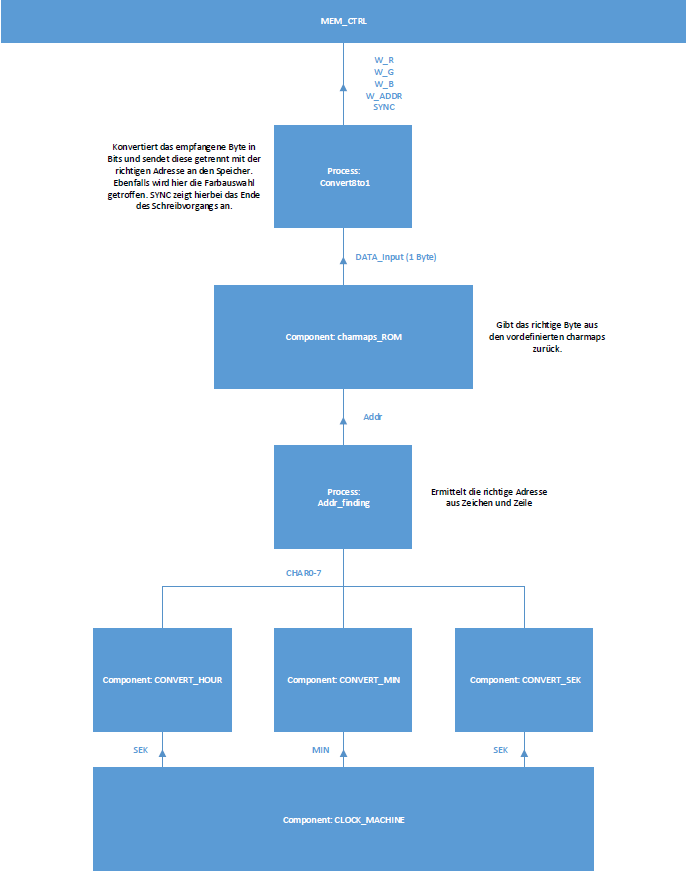
\includegraphics[scale = 0.44]{blockdiagramm}
	\caption{Schematische Darstellungder Komponente IMG\_CREATE}
	\label{blockdiagramm}
\end{figure}
Durch die Vorgabe der anderen Komponenten war bereits ein gewisser Weg vorgegeben. Einige Unterschiede könnten lediglich in der Programmierung 
entstehen. Die Trennung in zwei Prozesse ist hierbei sinnvoll da beide von unterschiedlichen Takten beeinflusst werden. Außerdem haben beide einen 
anderen Kontext: "`Addr\_finding" \,das Ansprechen der Komponenten "`charmaps\_ROM" \,und "`Convert8to1"\, das Weiterleiten der Farben mit der 
richtigen Adresse an den Speichercontroller.


\subsection{Umgesetzte Lösung}
Der grundsätzliche Aufbau wird in der folgenden Grafik \ref{blockdiagramm} anhand eines Blockdiagramms dargestellt.

Dabei wird die gesamte Einheit unterhalb von "`MEM\_CTRL" \,als "`IMG\_Creation" \,beschrieben. Diese besteht aus den Komponenten \,
"`CLOCK\_MACHINE"\,,
"`CONVERT" \,und "`charmaps\_ROM",\, sowie den Prozessen "`Addr\_finding" \,und "`Convert8to1". Der Grundaufbau der Uhr beginnt dabei in der 
"`CLOCK\_MACHINE", welche die Zahlen der Uhr festlegt. Diese werden dann von der Komponente "`CONVERT" \,in ASCII umgewandelt. Mit diesen 
Ausgangswerten beginnt der Prozess "`Addr\_finding". Dort werden die letzten sechs Zeichen der Bitfolge mit 16 multipliziert. Anschließend 
wird noch ein Zähler für die aktuelle Zeile hinzuaddiert. Dabei wird immer zuerst die erste Zeile des ersten Zeichens, dann die erste 
Zeile des zweiten Zeichens bearbeitet, da dies dem Lesevorgang aus dem Speicher heraus entspricht.

\begin{figure}[htbp]
	\centering
	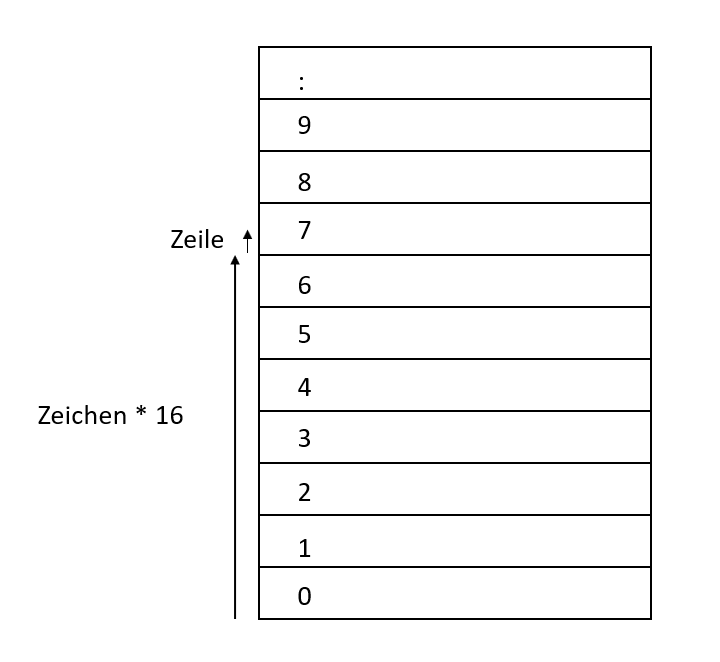
\includegraphics[scale = 0.4]{Aufbaucharmaps}
	\caption{Charmap Aufteilung und Adresse}
	\label{charmaps}
\end{figure} 
 
Dies ist dadurch möglich, da die letzten sechs Bit des ASCII-Codes genau der Adresse der Charmaps entsprechen. Die genaue Charmapaufteilung ist in 
der Grafik \ref{charmaps} zu sehen. Jedes Kästchen/Zeichen besteht dabei aus 16 Zeilen mit einer Länge von einem Byte. Nach einem kompletten 
Durchlauf der Zeichenfolge werden die Zähler zurückgesetzt. Da jedoch die Konvertierung im Prozess "`Convert8to1" \,im Takt der W\_CLk erfolgt muss 
Hier der Takt acht mal langsamer sein. Dies wurde über einen weiteren Zähler realisiert. Dieser Zähler gibt außerdem den Takt für die Komponente 
"`charmaps\_ROM" \,vor, damit dem Process "`Convert8to1" \,genügend Zeit bleibt das ankommende Byte auch zu verarbeiten. Um die durch die zeitlichen 
Diskrepanzen entstehenden Standardwerte der Komponente "`charmaps\_ROM"\, auszugleichen wird ein Standardwert gewählt der in keiner Bytekombination 
vorkommt, in diesem Fall "`12". Diese wird dann im Prozess "`Convert8to1" \,ausgefiltert.
Dort wird dann das ankommende Byte von der Stelle 7 bis zur Stelle 0 durchgegangen und jeweils im normalen Takt eine 
Farbkombination in den Speicher geschrieben. Die Adresse wird dabei mit Konstanten verrechnet, die die Abstände zum Bildschirmrand festlegen, siehe 
\ref{bildschirm}. Die Adresse wird dabei nach folgender Gleichung berechnet: 
{\centering
\newline
$\text{Pixeladresse} = (\text{Vertikaler Abstand} * 
\text{horizontaler Maximalwert}) + (\text{Zähler Zeilen} * \text{horizontaler Maximalwert}) + \text{ Horizontaler Abstand } + 
\text{Bit innerhalb des Zeichens}\newline (\text{Zeichen} * 8)$
\newline 
}
\begin{figure}[htbp]
	\centering
	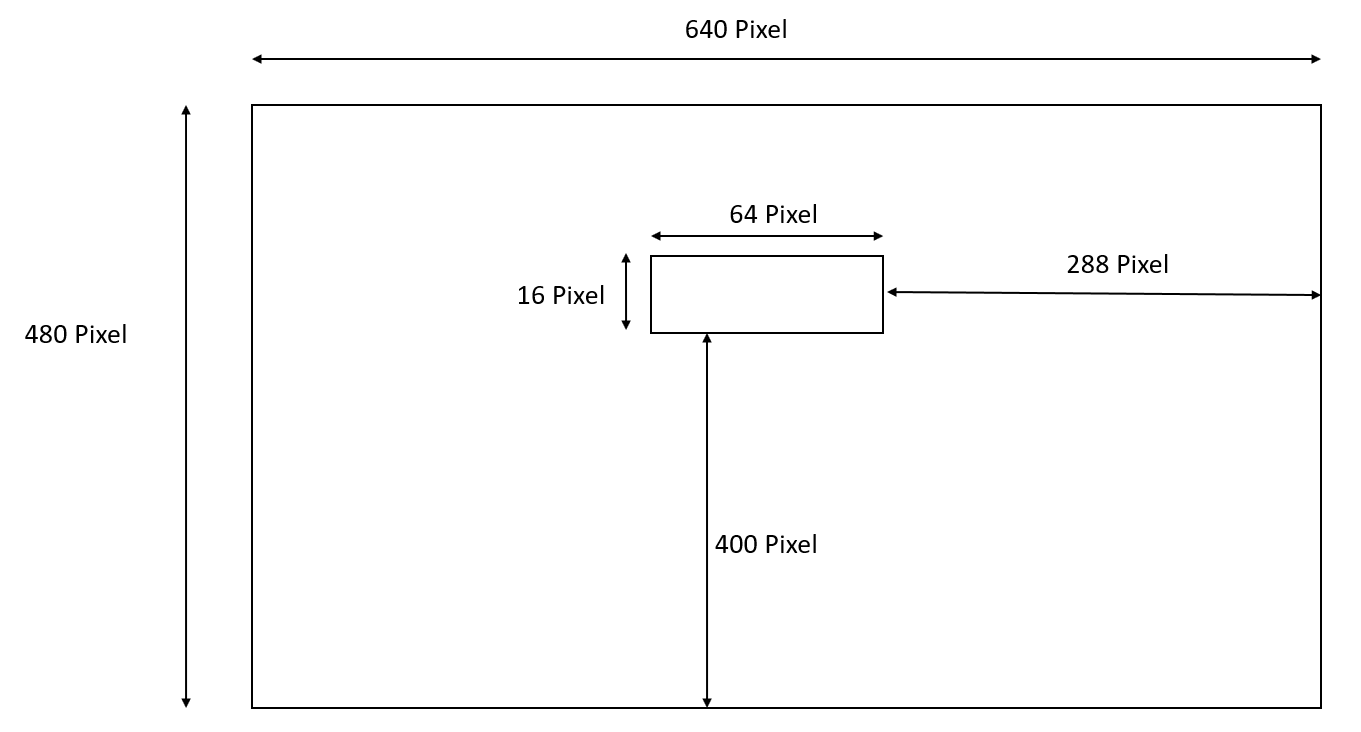
\includegraphics[scale = 0.38]{AufbauBildschirmspeicher}
	\caption{Aufteilung Bildschirm bzw. Adressraum}
	\label{bildschirm}
\end{figure} 
Dadurch wird die richtige Speicherzelle mit den 12 Bit des Farbcodes gefüllt, vier Bit für jede Farbe. 
Dieser reicht daher pro Farbe von 0 bis 255. Beim Schreibvorgang wird somit nur der Bereich beschrieben in dem die Uhr auch zu sehen ist. 
Daher werden auch nur $16 \text{ Zeilen } * 8 \text{ Zeichen } * 8 \text{ Byte } = 1024 \text{ Speicherzellen }$ direkt angesprochen, wie in \ref{bildschirm} zu sehen ist.
%vOFFSET+("00000" & Count_Zeile_write)* h_max)+ hOFFSET+ Count_Convert2+Count_Char_write*"8"
%pixeladdr = vOFFSET+Count_Zeile*(h_max)+hOFFSET+Count_Convert(Count_Char*8)  
Dabei wurde auch noch eine Funktion implementiert die die Farben verändert. So wird immer eine Farbe von dem Wert "`0100"\, bis zum Maximalwert erhöht. 
Der Grundwert muss dabei ausreichend hoch angesetzt werden, damit dennoch eine Farbe zu sehen ist. 



\subsection{Mögliche Erweiterungen}
Die Anzeige könnte um eine Anzeige in Millisekunden erweitert werden. Dies ist ebenfalls in die andere Richtung möglich (Tage/Wochen/etc.). 
Dazu müsste allerdings die Komponente "`CLOCK\_MACHINE"\, um die richtigen Zähler erweitert werden. Ebenfalls verändert werden müsste der Prozess 
"`Addr\_finding"\, und zwar um zwei weitere Zustände des Zählers "`Count\_Char". Die Adresse würde sich dabei nicht unterscheiden, da die gleichen 
Zeichen aus "`charmaps\_ROM" \,verwendet werden.\newline
Eine weitere Erweiterung wäre die Ausgabe der Uhr in einem bewegten Modus, wie ältere Bildschirmschoner. Dazu müsste ein weitere Zähler eingefügt 
werden, der nach einem vollständigen Schreibvorgang weiter zählt und dabei die Adresse verändert. Dies bewirkt allerdings nur eine Verschiebung in 
horizontaler Richtung. Zusätzlich könnte auch noch ein zweiter Zähler eingeführt werden, der in vertikaler Richtung weiter zählt, nach dem 
Modus: \newline $\text{Vertikaler Zähler} * \text{horizontaler Maximalwert} = \text{Vertikale Verschiebung}$\newline Dadurch würde dann eine diagonale Verschiebung erfolgen. Außerdem sollten noch Grenzen festgelegt 
werden, die verhindern, dass die Uhr nicht mehr zu sehen ist, da sie in einem Bereich angezeigt wird, der duch die Komponente "`Blank\_Check"\, nicht an 
den Bildschirm gesendet wird. Da die Grenzen der Uhr fest vorgegeben sind muss dazu lediglich eine Abfrage erfolgen.
Bei einer sich bewegenden Uhr müssen allerdings alle nicht beschriebenen Pixel wieder auf "`0" \,gesetzt werden, da ansonsten die Überbleibsel des 
vorherigen Schreibvorgangs noch zu sehen sind.

\subsection{Zusammenfassung}

\pagebreak
% ----------------------------------------------------------------------------------
% Kapitel 2: Speicherverwaltung Michael Braun
% ----------------------------------------------------------------------------------
\section{Speicherverwaltung}
\subsection{Überblick}


\pagebreak
% ----------------------------------------------------------------------------------
% Kapitel 3: Timing und Blank\_Check Korbinian Federholzner
% ----------------------------------------------------------------------------------
\section{Timing und Blank\_Check}
\subsection{Überblick}

\subsection{}


\pagebreak
% ----------------------------------------------------------------------------------
% Kapitel: Fazit und Ausblick
% ----------------------------------------------------------------------------------
\section{Fazit und Ausblick}



\pagebreak


% ----------------------------------------------------------------------------------
% Kleine Einführung in LaTeX-Elemente
% ----------------------------------------------------------------------------------
%\section{\LaTeX-Elemente}
%Dieser Abschnitt beinhaltet lediglich einige Informationen über \LaTeX-Distributionen, Editoren und \LaTeX-Elemente, die Ihnen beim Einstieg in das \LaTeX-Textsatzsystem helfen sollen.

%\subsection{\LaTeX-Distributionen nach Betriebssystemen}

%\subsubsection{\LaTeX-Distributionen}
%Folgende Haupt-\LaTeX-Distributionen stehen Ihnen zur Verfügung:
%\begin{itemize}
%  \item Windows:\quad \texttt{MiKTeX}\quad Webseite:\quad\url{http://www.miktex.org}
%  \item Linux/Unix:\quad \texttt{TeX Live}\quad Webseite:\quad\url{http://tug.org/texlive/}
%  \item Mac OS:\quad \texttt{MacTeX}\quad Webseite:\quad\url{http://www.tug.org/mactex/}
%\end{itemize}

%\subsubsection{\LaTeX-Editoren}
%Auf folgenden Webseiten können Sie einige hilfreiche \LaTeX-Editoren finden:
%\begin{itemize}
%  \item Windows/Linux/Mac OS: \url{http://www.xm1math.net/texmaker/}
%  \item Windiws: \url{http://www.texniccenter.org/}
%  \item Mac OS: \url{http://pages.uoregon.edu/koch/texshop/}
%\end{itemize}

%Falls bei den oben genannten Editoren kein passender vorhanden war, findet sich auf Wikipedia eine Zusammenstellung vieler weiterer \LaTeX-Editoren:\\
%\url{https://en.wikipedia.org/wiki/Comparison_of_TeX_editors}

%Für die PDF-Anzeige empfiehlt sich SumatraPDF: \\ 
%\url{https://www.sumatrapdfreader.org/free-pdf-reader.html}.


%\subsection{Bilder}
%Zum Einfügen eines Bildes, siehe Abbildung \ref{fig:reversi01}, werden die \texttt{minipage}-Umgebung und der Befehl \texttt{$\backslash$includegraphics} genutzt, da die Bilder so gut positioniert und einfach integriert und skaliert werden können.

%\vspace{1em}
%\begin{minipage}{\linewidth}
%	\centering
%	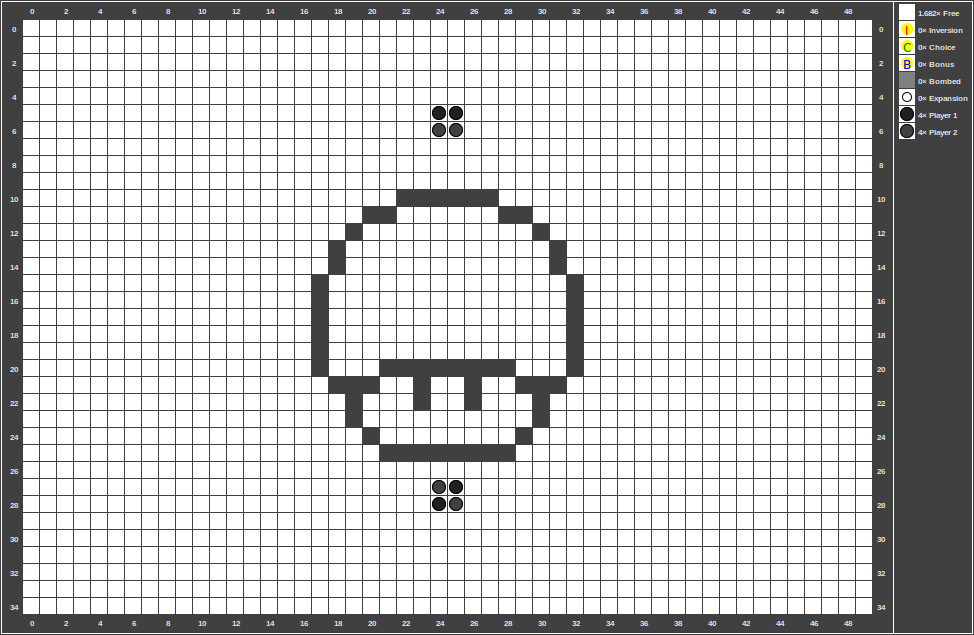
\includegraphics[width=0.5\linewidth]{pics/gamefield01.png}
%	\captionof{figure}[Spielfeld 01]{Unbespieltes Spielfeld}
%	\label{fig:reversi01}
%\end{minipage}


%Nachdem das Spielt gestartet wurde und beide Spielphasen durchlaufen wurden, siegt schließlich der Spieler mit der Farbe rot.

%\vspace{1em}
%\begin{minipage}{\linewidth}
%	\centering
%	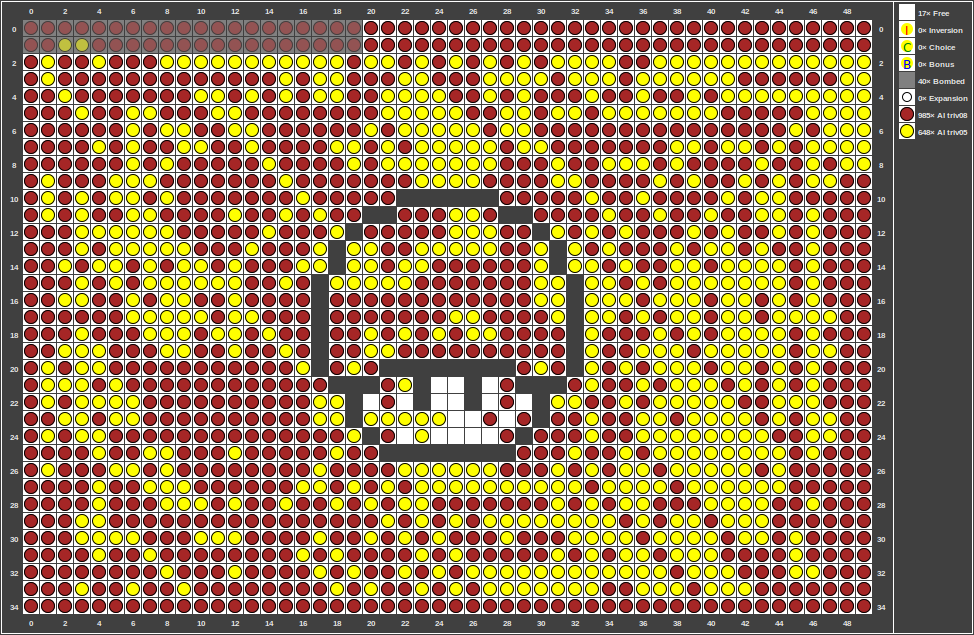
\includegraphics[width=0.5\linewidth]{pics/gamefield02.png}
%	\captionof{figure}[Spielfeld 02]{Finales Spielfeld}
%	\label{fig:reversi2}
%\end{minipage}


%\subsection{Tabellen}
%In diesem Abschnitt wird eine Tabelle (siehe Tabelle \ref{tab:beispiel}) dargestellt.

%\vspace{1em}
%\begin{table}[!h]
%	\centering
%	\begin{tabular}{|l|l|l|}
%		\hline
%		\textbf{Name} & \textbf{Name} & \textbf{Name}\\
%		\hline
%		1 & 2 & 3\\
%		\hline
%		4 & 5 & 6\\
%		\hline
%		7 & 8 & 9\\
%		\hline
%	\end{tabular}
%	\caption{Beispieltabelle}
%	\label{tab:beispiel}
%\end{table}


%\subsection{Auflistung}
%Für Auflistungen wird die \texttt{enumerate}- oder \texttt{itemize}-Umgebung genutzt.

%\begin{itemize}
%	\item Nur
%	\item ein
%	\item Beispiel.
%\end{itemize}

%\subsection{Listings}
%Sehen Sie in Listing \ref{lst:helloworld} ein Beispiel für das Einbinden von Quellcode mit Syntax-Highlighting.

%\vspace{1em}
%\lstinputlisting[caption=Brute Force-Ansatz für das MaxTeilsum2D-Problem, label=lst:maxTeilsumZweiD,basicstyle=\ttfamily\scriptsize]{code/maxTeilsum2DBruteForce.txt}
%\lstinputlisting[caption=Hello World Program, label=lst:helloworld,basicstyle=\ttfamily\scriptsize]{code/helloworld.c}

%\subsection{Gleichungen}
%Formatierung von Formeln:
%\begin{itemize}
%  \item Formelzeichen sind in kursiv zu setzen
%  \item Zahlen, Einheiten und Funktionsnamen sind in normaler Schriftart zu setzen (nicht kursiv)
%  \item Häufig wird fälschlicherweise das Symbol * als Multiplikationszeichen verwendet
%  \item Zwischen Zahl und Einheit ist ein Leerzeichen zu setzen
%\end{itemize}

%Frequency Modulation (FM) is a wireless transmission system patent-registered by Edwin H. Armstrong in 1933. It is still widespread in the area of audio broadcasting today. In case of the frequency modulation the amplitude of the desired message signal varies the frequency (the argument) of the sinusoidal carrier. The general FM oscillation is formulated with 
%\begin{equation}
%u_{\textrm{FM}}(t)= a_0 \cos(\Psi(t)+\varphi_0) 
%\label{eqn:fmosc}
%\end{equation}

%To simplify matters, only an one-tone modulation signal is considered to characterize the spectrum of FM-signals at first
%\begin{multline}
%u_{\textrm{FM}}(t)=\hat u_T \cdot [J_0(\eta)\cos\omega_Tt + \sum_{n=1}^{+\infty} J_n(\eta) \cdot (\cos[(\omega_T+n\omega_1)t]+(-1)^n \cos[(\omega_T-n\omega_1)t])] 
%\\ \ \mbox{with Bessel functions:} \ J_n(\eta)= \frac{(-1)^n}{\pi} \int_0^{\pi} e^{j\eta\sin x} \cdot \cos(nx) dx 
%\end{multline}

%\subsection{Verwendung von Abkürzungen}
%Die Abkürzungen können so verwendet werden:
%Beim ersten Mal der Verwendung (vgl. Einleitung) wird die Abkürzung ausgeschrieben \ac{BA}. Beim zweiten Mal oder folgenden Malen wird nur noch die Abkürzung verwendet \ac{BA}.
%Aber setzen Sie Abkürzungen sparsam ein.

%\subsection{Tipps}
%Die Quellen befinden sich in der Datei \textit{quellen.bib}. 
%Alle Literaturangaben müssen im Text referenziert werden. Die höchstwertigen Quellen stellen dabei Zeitschriftenartikel \cite{Laprie2004}, gefolgt von Konferenzbeiträgen \cite{Agrou2011}, Patenten \cite{Grisenthwaite2012}, Standards \cite{ARINC2005}, Fachbüchern \cite{Kopetz2011},  Datenblättern \cite{Freescale2015}, Techreports und White-Papern \cite{Aswadhati2011} und zuletzt Onlinequellen \cite{Xil2010} dar.

\pagebreak



% ----------------------------------------------------------------------------------------------------------
% Anhang
% ----------------------------------------------------------------------------------------------------------
\pagenumbering{Roman}
\setcounter{page}{1}
\lhead{Anhang \thesection}

\begin{appendix}
\section*{Anhang}
\phantomsection
\addcontentsline{toc}{section}{Anhang}
\addtocontents{toc}{\vspace{-0.5em}}

%\section{Domändenmodell}
%Ein toller Anhang.


%\subsection*{Screenshot}
%\label{app:screenshot}
%Unterkategorie, die nicht im Inhaltsverzeichnis auftaucht.
%\pagebreak

\end{appendix}


% ----------------------------------------------------------------------------------------------------------
% Abkürzungsverzeichnis
% ----------------------------------------------------------------------------------------------------------
\section{Abkürzungsverzeichnis}
\begin{acronym}[KDE]
	\acro{BA}[BA]{Bachelorarbeit}
	\acro{MA}[MA]{Masterarbeit}
\end{acronym}
\pagebreak


% ----------------------------------------------------------------------------------------------------------
% Abbildungsverzeichnis (optional)
% ----------------------------------------------------------------------------------------------------------
\section {Abbildungsverzeichnis}
\listoffigures
\pagebreak

% ----------------------------------------------------------------------------------------------------------
% Tabellenverzeichnis (optional)
% ----------------------------------------------------------------------------------------------------------
%\listoftables
%\pagebreak

% ----------------------------------------------------------------------------------------------------------
% Listingsverzeichnis (optional; Code nur, wenn wirklich sinnvoll und wichtig)
% ----------------------------------------------------------------------------------------------------------
%\lstlistoflistings
%\pagebreak

% ----------------------------------------------------------------------------------------------------------
% Eidestattliche Erklärung
% ----------------------------------------------------------------------------------------------------------
%\addsec{Eidesstattliche Erklärung}
%...
%\pagebreak

% ----------------------------------------------------------------------------------------------------------
% Literatur
% ----------------------------------------------------------------------------------------------------------
\renewcommand\refname{Literaturverzeichnis}
\lhead{}
%\bibliographystyle{alpha}
\bibliographystyle{ieeetr}
\bibliography{quellen}
\pagebreak

% ----------------------------------------------------------------------------------------------------------
% Inhalt des Datenträgers
% ----------------------------------------------------------------------------------------------------------
\addsec{Inhalt des Datenträgers}
\begin{itemize}
	\item $\ldots$
	\item $\ldots$
\end{itemize}
\pagebreak

\end{document}
